%=========================================================
\chapter{Modelo de la interacción}	
\label{cap:modInteraccion}

Este capítulo describe los detalles de la interacción del usuario con el sistema **Taimotla**, abordando los principios de usabilidad, ergonomía y arquitectura de la información de la interfaz. Se detalla el modelo de navegación y se especifican las pantallas del sistema junto con el catálogo de mensajes.

%---------------------------------------------------------
\section{Modelo de navegación}

La navegación entre las pantallas del sistema se muestra en el mapa del sitio de la figura~\ref{fig:mapaNavegacion}. El acceso inicial se da a través de la pantalla de inicio de sesión. Una vez autenticado, el sistema bifurca el flujo de navegación de forma estricta según el rol del usuario (Director, Coordinador o Especialista), restringiendo la consulta de pantallas cruzadas para asegurar la confidencialidad de los datos.

\begin{figure}[htbp!]
	\begin{center}
		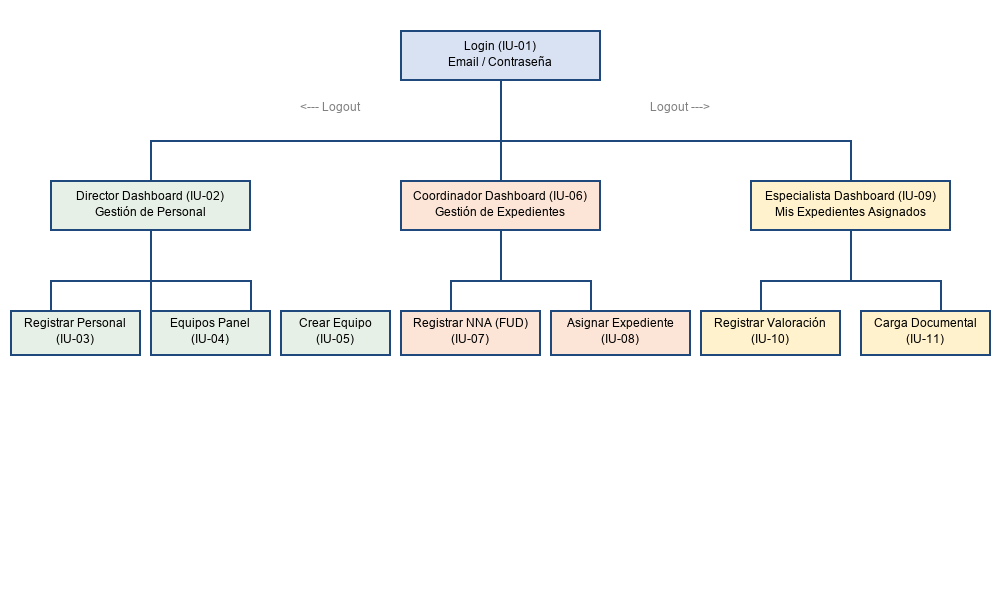
\includegraphics[width=.9\textwidth]{images/mapa_navegacion_taimotla}
		\caption{Mapa de navegación del sistema Taimotla.}
		\label{fig:mapaNavegacion}
	\end{center}
\end{figure}

A continuación se detalla la especificación de las pantallas principales del sistema:

%--------------------------------------
\section{IU23 Pantalla de Control de Acceso}

\subsection{Objetivo}
	Controlar el acceso seguro al sistema Taimotla mediante la validación de las credenciales (correo electrónico y contraseña) del personal de la Fundación, de modo que cada usuario acceda únicamente al módulo de acuerdo con su rol autorizado.

\subsection{Diseño}
	Esta pantalla \IUref{IU23}{Pantalla de Control de Acceso} (ver figura~\ref{IU23}) es la interfaz inicial que se muestra al acceder a la dirección URL de la aplicación web. El usuario debe capturar su dirección de correo electrónico institucional y su contraseña de acceso secreta.

\IUfig[.45]{Login}{IU23}{Pantalla de Control de Acceso.}

\subsection{Salidas}
	\begin{Citemize}
		\item Redirección automática al panel correspondiente:
			\begin{itemize}
				\item Módulo del Director (Administración general y gestión de equipos).
				\item Módulo del Coordinador (Asignación y visualización de expedientes).
				\item Módulo del Especialista (Consulta de expediente, registro de valoraciones e historial).
			\end{itemize}
	\end{Citemize}

\subsection{Entradas}
	\begin{itemize}
		\item Correo electrónico del usuario (ej. \texttt{director@fundacion.org}).
		\item Contraseña del usuario.
	\end{itemize}

\subsection{Comandos}
\begin{itemize}
	\item \IUbutton{Entrar}: Ejecuta la validación de las credenciales del usuario en la base de datos de acuerdo con la regla de negocio \hyperlink{BR-03}{BR-03}. Si los datos son correctos, inicia la sesión e ingresa al sistema.
	\item \IUbutton{¿Olvidaste tu contraseña?}: Enlace que redirige a la pantalla de recuperación de credenciales mediante el correo electrónico registrado.
\end{itemize}

\subsection{Mensajes}
\begin{Citemize}
	\item {\bf MSG-02} (Usuario no registrado): Se muestra cuando el correo electrónico ingresado no coincide con ninguna cuenta registrada y activa en el sistema.
	\item {\bf MSG-04} (Error de inicio de sesión): Se muestra cuando la contraseña no coincide con la guardada para el correo especificado.
	\item {\bf MSG-03} (Cuenta inactiva): Se muestra si el usuario intenta ingresar con una cuenta que ha sido temporalmente deshabilitada por el Director.
\end{Citemize}

%--------------------------------------
\section{IU24 Pantalla de Gestión de Personal}

\subsection{Objetivo}
	Permitir al Director de la Fundación administrar de forma centralizada las cuentas, especialidades y estados de acceso del personal multidisciplinario y operativo.

\subsection{Diseño}
	Esta pantalla \IUref{IU24}{Pantalla de Gestión de Personal} (ver figura~\ref{IU24}) es accesible únicamente para el rol de Director General. Presenta un listado tabular que detalla el personal registrado, mostrando su CURP, nombre, rol en la Fundación (Coordinador o Especialista Abogado, Médico, Psicólogo, Trabajador Social), cédula profesional, fecha de alta y estado de cuenta (Habilitado/Deshabilitado).
	Incluye controles superiores para buscar personal por nombre o CURP y filtros de selección por especialidad.

\IUfig[.55]{default}{IU24}{Pantalla de Gestión de Personal.}

\subsection{Salidas}
	\begin{Citemize}
		\item Tabla dinámica con el personal registrado y sus datos laborales.
		\item Notificaciones informativas de estado de cuenta.
	\end{Citemize}

\subsection{Entradas}
	\begin{itemize}
		\item Filtro de búsqueda (por CURP o nombre del empleado).
		\item Selección de filtro por Rol o Especialidad.
	\end{itemize}

\subsection{Comandos}
	\begin{itemize}
		\item \IUbutton{Registrar Personal}: Abre el formulario de registro de nuevo personal bajo las validaciones de las reglas \hyperlink{BR-06}{BR-06}, \hyperlink{BR-07}{BR-07} y \hyperlink{BR-08}{BR-08}.
		\item \IUbutton{Editar}: Redirige a la pantalla de edición de datos personales del colaborador seleccionado.
		\item \IUbutton{Desactivar/Activar}: Cambia de forma lógica el estado del empleado en la base de datos (Habilitado/Deshabilitado). Las cuentas deshabilitadas perderán acceso inmediato al sistema según la regla \hyperlink{BR-03}{BR-03}.
	\end{itemize}

\subsection{Mensajes}
	\begin{Citemize}
		\item {\bf MSG-09} (Operación exitosa): Confirmación cuando se guarda un registro o se cambia el estado de la cuenta.
	\end{Citemize}
%--------------------------------------

%--------------------------------------
\section{IU25 Pantalla de Asignación de Casos}

\subsection{Objetivo}
	Permitir a los Coordinadores de Caso asociar un expediente digital de NNA recién registrado a un equipo multidisciplinario específico de especialistas para iniciar la fase de diagnósticos clínicos y valoraciones.

\subsection{Diseño}
	Esta pantalla \IUref{IU25}{Pantalla de Asignación de Casos} (ver figura~\ref{IU25}) se estructura en dos paneles principales:
	\begin{enumerate}
		\item **Panel Izquierdo (Casos Pendientes):** Muestra el listado de expedientes en estado "Creado" con el folio del caso y la fecha de apertura.
		\item **Panel Derecho (Equipos Multidisciplinarios):** Presenta una lista de los equipos configurados por la Dirección, mostrando su nombre y la lista de especialistas (Médico, Psicólogo, Abogado, Trabajador Social) asignados.
	\end{enumerate}
	El Coordinador de Caso debe seleccionar un expediente del panel izquierdo y un equipo del panel derecho para habilitar el botón de asignación.

\IUfig[.55]{default}{IU25}{Pantalla de Asignación de Casos.}

\subsection{Salidas}
	\begin{Citemize}
		\item Listado de expedientes sin equipo asignado.
		\item Listado de equipos de trabajo registrados.
	\end{Citemize}

\subsection{Entradas}
	\begin{itemize}
		\item Selección de expediente de NNA.
		\item Selección del equipo multidisciplinario responsable.
	\end{itemize}

\subsection{Comandos}
	\begin{itemize}
		\item \IUbutton{Asignar caso}: Ejecuta la vinculación en base de datos. Transiciona el expediente de "Creado" a "En Diagnóstico" y notifica a los especialistas implicados en el equipo según las reglas de negocio \hyperlink{BR-01}{BR-01} y \hyperlink{BR-02}{BR-02}.
	\end{itemize}

\subsection{Mensajes}
	\begin{Citemize}
		\item {\bf MSG-09} (Operación exitosa): Confirmación cuando se asocia con éxito el caso al equipo multidisciplinario.
		\item {\bf MSG-04} (Error en entrada): Se muestra si el Coordinador presiona "Asignar caso" sin haber seleccionado previamente un menor o un equipo.
	\end{Citemize}
%--------------------------------------

%--------------------------------------
\section{IU26 Pantalla de Expediente Único de NNA}

\subsection{Objetivo}
	Permitir al personal multidisciplinario visualizar y actualizar toda la información clínica, legal, familiar, social y los documentos digitalizados obligatorios de las NNA asignados a su equipo.

\subsection{Diseño}
	Esta pantalla \IUref{IU26}{Pantalla de Expediente Único de NNA} (ver figura~\ref{IU26}) unifica toda la información del caso mediante una interfaz estructurada en pestañas lógicas:
	\begin{description}
		\item[Pestaña General (FUD):] Muestra los datos de identidad básica (CURP, nombre, apodo), nacionalidad, etnia y datos del tutor o familiares de la NNA.
		\item[Pestaña Hecho Victimal:] Registro y consulta del folio de reporte, nombre del caso, fecha de detención, narración del suceso y nombre de la madre víctima del feminicidio.
		\item[Pestaña Documentación:] Sección para adjuntar y validar los documentos de identidad digitalizados. El Abogado del caso puede cargar archivos PDF/PNG/JPG que son validados bajo las restricciones de la regla \hyperlink{BR-10}{BR-10}.
		\item[Pestaña Valoración Multidisciplinaria:] Pestañas internas para cada área técnica (Abogado: Legal; Médico: Salud Física; Psicólogo: Salud Emocional; Trabajador Social: Entorno Sociofamiliar). Permite agregar notas de diagnóstico y adjuntar peritajes especializados.
		\item[Pestaña Plan de Restitución (PRD):] Visualización de las medidas de protección asignadas, su estado de ejecución y alertas visuales de plazos límite de vigencia.
	\end{description}

\IUfig[.55]{default}{IU26}{Pantalla de Expediente Único de NNA.}

\subsection{Salidas}
	\begin{Citemize}
		\item Ficha técnica unificada y descargable del menor (FUD unificado).
		\item Historial cronológico de notas de evolución y valoraciones de los especialistas.
		\item Lista de documentos validados cargados en el expediente.
	\end{Citemize}

\subsection{Entradas}
	\begin{itemize}
		\item Notas diagnósticas y reportes periciales por especialista.
		\item Archivos digitales digitalizados (Acta de nacimiento, CURP, Cartilla de salud).
	\end{itemize}

\subsection{Comandos}
	\begin{itemize}
		\item \IUbutton{Subir Archivo}: Permite seleccionar y adjuntar un archivo digital. Valida formato y peso máximo según la regla de negocio \hyperlink{BR-10}{BR-10}.
		\item \IUbutton{Guardar Diagnóstico}: Guarda la valoración redactada en la pestaña de especialidad correspondiente asociando la fecha y firma del especialista activo.
		\item \IUbutton{Validar Acta}: Comando exclusivo del Abogado para marcar el acta de nacimiento del expediente como "Verificada", cumpliendo la regla \hyperlink{BR-04}{BR-04}.
	\end{itemize}

\subsection{Mensajes}
	\begin{Citemize}
		\item {\bf MSG-09} (Operación exitosa): Confirmación cuando se guarda un diagnóstico o se sube un archivo con éxito.
		\item {\bf MSG-04} (Error de formato): Alerta si se intenta subir un archivo que excede 5MB o formato no compatible (rompiendo \hyperlink{BR-10}{BR-10}).
		\item {\bf MSG-02} (Permisos inválidos): Se muestra si un especialista intenta registrar diagnósticos en un caso que no tiene asignado.
	\end{Citemize}
%--------------------------------------

%--------------------------------------
\section{IU27 Pantalla de Registro de Equipo de Trabajo}

\subsection{Objetivo}
	Permitir al Director General configurar y registrar un nuevo equipo multidisciplinario asignándole un nombre descriptivo, un coordinador de caso activo y seleccionando especialistas disponibles.

\subsection{Diseño}
	Esta pantalla \IUref{IU27}{Pantalla de Registro de Equipo de Trabajo} (ver figura~\ref{IU27}) se organiza en dos áreas principales:
	\begin{enumerate}
		\item **Encabezado y Datos Generales (Formulario):** Contiene la caja de entrada para el nombre del equipo y la lista de selección con los coordinadores activos disponibles en el sistema.
		\item **Panel de Personal (Cuadrícula):**
			\begin{itemize}
				\item **Columna Izquierda (Disponible):** Muestra tarjetas de empleados agrupados por especialidades (Abogados, Médicos, Psicólogos y Trabajadores Sociales) que no estén asignados a otro equipo activo. Cada tarjeta incluye un botón \IUbutton{+} para agregarlo.
				\item **Columna Derecha (Integrantes):** Muestra una tabla con la lista de personal seleccionado para conformar el equipo con la opción de eliminarlos mediante el botón \IUbutton{X}.
			\end{itemize}
	\end{enumerate}

\IUfig[.55]{default}{IU27}{Pantalla de Registro de Equipo de Trabajo.}

\subsection{Salidas}
	\begin{Citemize}
		\item Catálogo de coordinadores activos y personal operativo disponible sin equipo asignado.
		\item Lista de integrantes agregados dinámicamente con su rol.
	\end{Citemize}

\subsection{Entradas}
	\begin{itemize}
		\item Nombre del equipo (Texto obligatorio).
		\item Selección del Coordinador (Menú desplegable obligatorio).
		\item Selección de especialistas operativos a integrar en el equipo.
	\end{itemize}

\subsection{Comandos}
	\begin{itemize}
		\item \IUbutton{+}: Agrega al especialista seleccionado de la lista de disponibles a la tabla de integrantes (máximo 4 y sin duplicidad de especialidades).
		\item \IUbutton{X}: Remueve al especialista seleccionado de la tabla de integrantes y lo regresa a la lista de disponibles.
		\item \IUbutton{AGREGAR EQUIPO}: Envía la información capturada al servidor para registrar el equipo y sus asociaciones en la base de datos.
	\end{itemize}

\subsection{Mensajes}
	\begin{Citemize}
		\item {\bf MSG-09} (Operación exitosa): Confirmación tras registrar exitosamente el equipo en el sistema.
		\item {\bf MSG-04} (Error de validación): Alerta si falta capturar algún dato obligatorio o la composición del equipo no cumple con el número mínimo de integrantes (2).
	\end{Citemize}
%--------------------------------------

%--------------------------------------
\section{IU28 Pantalla de Gestión de Equipos}

\subsection{Objetivo}
	Permitir al Director General visualizar la composición de los equipos multidisciplinarios activos y realizar operaciones de modificación en línea (reasignación de coordinador, altas y bajas de especialistas o disolución de equipos).

\subsection{Diseño}
	Esta pantalla \IUref{IU28}{Pantalla de Gestión de Equipos} (ver figura~\ref{IU28}) presenta un listado de tarjetas de los equipos activos. Cada tarjeta cuenta con dos estados visuales:
	\begin{enumerate}
		\item **Modo Vista:** Muestra el nombre del equipo, el nombre del coordinador asignado y una tabla con los integrantes activos y sus roles específicos.
		\item **Modo Edición:** Se activa al presionar el botón de edición \IUbutton{Editar} y permite modificar en línea:
			\begin{itemize}
				\item El coordinador asignado mediante una lista de selección.
				\item Remover integrantes utilizando el botón de baja \IUbutton{Quitar} en cada renglón.
				\item Eliminar por completo el equipo mediante el botón \IUbutton{Eliminar Equipo}.
			\end{itemize}
	\end{enumerate}
	Adicionalmente, bajo el botón \IUbutton{+} se despliega un panel flotante de personal operativo disponible agrupado por rol para agregar miembros al equipo que posea menos de 4 integrantes.

\IUfig[.55]{28}{IU28}{Pantalla de Gestión de Equipos.}

\subsection{Salidas}
	\begin{Citemize}
		\item Listado de tarjetas de equipos multidisciplinarios activos con su personal asignado.
		\item Panel de personal especialista disponible para adición en línea.
	\end{Citemize}

\subsection{Entradas}
	\begin{itemize}
		\item Selección de coordinador de la lista desplegable.
		\item Selección de especialista disponible a integrar.
	\end{itemize}

\subsection{Comandos}
	\begin{itemize}
		\item \IUbutton{Editar}: Alterna la tarjeta de equipo entre Modo Vista y Modo Edición.
		\item \IUbutton{+}: Abre/cierra el panel de personal disponible para agregar integrantes.
		\item \IUbutton{Quitar}: Envía la solicitud para dar de baja de forma inmediata al miembro seleccionado del equipo.
		\item \IUbutton{Eliminar Equipo}: Inactiva el equipo en base de datos y libera a todos sus integrantes cerrando su participación.
		\item \IUbutton{Cancelar}: Cierra el Modo Edición sin realizar cambios adicionales en la estructura del equipo.
	\end{itemize}

\subsection{Mensajes}
	\begin{Citemize}
		\item {\bf MSG-09} (Operación exitosa): Confirmación cuando se guarda algún cambio de composición, reasignación o disolución.
		\item Diálogo de Confirmación: Mensaje emergente del navegador (ej. ``¿Quitar a este miembro del equipo?'' o ``¿Estás seguro de querer eliminar el equipo seleccionado?'') para evitar acciones accidentales.
	\end{Citemize}
%--------------------------------------

%--------------------------------------
\section{IU29 Pantalla de Perfil de Usuario}

\subsection{Objetivo}
	Permitir al usuario autenticado (Director o Coordinador) consultar la información administrativa general asociada a su cuenta de acceso en el sistema Taimotla.

\subsection{Diseño}
	Esta pantalla \IUref{IU29}{Pantalla de Perfil de Usuario} (ver figura~\ref{IU29}) se estructura en una tarjeta de perfil centralizada que presenta la siguiente información del colaborador en modo de solo lectura:
	\begin{itemize}
		\item **Nombre Completo:** Nombre(s) y apellidos del usuario.
		\item **Rol Operativo:** Etiqueta visual indicando el rol en la Fundación (ej. Director de la Fundación o Coordinador de Caso).
		\item **Detalles de Registro:**
			\begin{itemize}
				\item Clave Única de Registro de Población (CURP).
				\item Fecha de ingreso o alta administrativa en la institución.
				\item Estado actual de la cuenta (activo, inactivo).
			\end{itemize}
	\end{itemize}

\IUfig[.45]{default}{IU29}{Pantalla de Perfil de Usuario.}

\subsection{Salidas}
	\begin{Citemize}
		\item Ficha de datos de identificación y registro del usuario conectado.
	\end{Citemize}

\subsection{Entradas}
	Ninguna (interfaz de consulta estática).

\subsection{Comandos}
	\begin{itemize}
		\item \IUbutton{Volver al Panel}: Redirige al usuario a la pantalla del Dashboard principal correspondiente a su rol.
		\item \IUbutton{Cambiar Contraseña}: Despliega una notificación sobre el estado de desarrollo de la función de actualización de credenciales.
	\end{itemize}

\subsection{Mensajes}
	\begin{Citemize}
		\item Alerta informativa: ``Funcionalidad de cambio de contraseña próximamente''.
	\end{Citemize}
%--------------------------------------

%--------------------------------------
\section{IU30 Pantalla de Modificación de Perfil de Personal}

\subsection{Objetivo}
	Permitir al Director General actualizar la información de identificación, nombre completo, contacto y dirección de residencia de un colaborador previamente registrado en el sistema.

\subsection{Diseño}
	Esta pantalla \IUref{IU30}{Pantalla de Modificación de Perfil de Personal} (ver figura~\ref{IU30}) presenta un formulario extenso dividido en tres grupos lógicos:
	\begin{enumerate}
		\item **Datos de Identificación:** Muestra la CURP del empleado (campo deshabilitado no modificable por seguridad), y permite editar el RFC, Sexo y la Fecha de Nacimiento.
		\item **Nombre Completo:** Cajas de entrada de texto para modificar el primer nombre (obligatorio), segundo nombre, primer apellido (obligatorio) y segundo apellido.
		\item **Contacto y Dirección:** Campos para actualizar el Correo Electrónico (obligatorio), Teléfono, Calle, Número Exterior, Colonia, Código Postal, Municipio y Estado.
	\end{enumerate}

\IUfig[.55]{default}{IU30}{Pantalla de Modificación de Perfil de Personal.}

\subsection{Salidas}
	\begin{Citemize}
		\item Formulario precargado con los datos actuales del colaborador consultados desde la base de datos.
	\end{Citemize}

\subsection{Entradas}
	\begin{itemize}
		\item RFC (Opcional, 13 caracteres máximo).
		\item Sexo (Selección obligatoria).
		\item Fecha de Nacimiento (Calendario obligatorio).
		\item Primer Nombre y Primer Apellido (Texto obligatorio).
		\item Correo electrónico (Texto obligatorio en formato de email).
		\item Datos de domicilio (Calle, Número exterior, Colonia, Municipio, Estado y Código Postal de 5 dígitos).
		\item Teléfono (Texto opcional).
	\end{itemize}

\subsection{Comandos}
	\begin{itemize}
		\item \IUbutton{Cancelar}: Aborta la edición del colaborador y redirige al usuario de vuelta al Dashboard del Director.
		\item \IUbutton{Guardar Todos los Cambios}: Envía el formulario para su validación en el servidor y actualización correspondiente en las tablas `persona` y `personal`.
	\end{itemize}

\subsection{Mensajes}
	\begin{Citemize}
		\item {\bf MSG-09} (Operación exitosa): Se muestra tras persistir correctamente los datos modificados en la base de datos.
		\item {\bf MSG-04} (Error de validación): Se muestra si algún campo obligatorio se envía vacío o la sintaxis de correo o RFC es incorrecta.
	\end{Citemize}
%--------------------------------------

%--------------------------------------
\section{IU31 Panel de Control del Coordinador}

\subsection{Objetivo}
	Proveer al Coordinador de Caso un espacio de trabajo centralizado que le permita visualizar el personal operativo activo e inactivo de la Fundación y acceder a las funciones de gestión del equipo multidisciplinario asignado a su cargo.

\subsection{Diseño}
	Esta pantalla \IUref{IU31}{Panel de Control del Coordinador} (ver figura~\ref{IU31}) comparte la estructura visual del panel del Director pero con un alcance más restringido. Se organiza en dos secciones principales:
	\begin{enumerate}
		\item \textbf{Sección ``Personal Operativo'' (Personal Activo):} Tablas agrupadas por especialidad (Abogados, Trabajadores Sociales, Médicos y Psicólogos) que muestran para cada persona su cédula profesional, CURP, nombre completo, especialidad o enfoque (según aplique) y estado de cuenta. Cada renglón incluye botones de acción para editar o deshabilitar la cuenta.
		\item \textbf{Sección ``Historial / Inactivos'':} Tabla con el personal cuyo estado es ``Inactivo'', mostrando nombre, CURP, rol original y la opción de re-habilitar la cuenta.
	\end{enumerate}

\IUfig[.55]{default}{IU31}{Panel de Control del Coordinador.}

\subsection{Salidas}
	\begin{Citemize}
		\item Tablas de personal activo agrupadas por especialidad con sus datos laborales.
		\item Tabla de historial de personal inactivo o dado de baja.
	\end{Citemize}

\subsection{Entradas}
	Ninguna (interfaz de consulta).

\subsection{Comandos}
	\begin{itemize}
		\item \IUbutton{Registrar Nuevo Personal}: Redirige al formulario de registro de un nuevo especialista operativo.
		\item \IUbutton{Editar} (icono de edición): Redirige a la pantalla de edición de datos del colaborador seleccionado (\IUref{IU30}{Pantalla de Modificación de Perfil}).
		\item \IUbutton{Deshabilitar} (icono de bloqueo): Cambia el estado lógico del empleado a ``Inactivo'' en la base de datos mediante un mensaje de confirmación del navegador.
		\item \IUbutton{Eliminar} (icono de eliminación): Elimina permanentemente el registro del empleado tras confirmación del navegador.
		\item \IUbutton{Habilitar Cuenta}: Reactiva un empleado de la sección de inactivos devolviendo su estado a ``Activo''.
	\end{itemize}

\subsection{Mensajes}
	\begin{Citemize}
		\item {\bf MSG-09} (Operación exitosa): Se muestra tras deshabilitar, habilitar o eliminar un registro de manera exitosa.
		\item Diálogo de confirmación del navegador: ``¿Deshabilitar cuenta?'' o ``¿Eliminar permanentemente?'' para prevenir acciones accidentales.
	\end{Citemize}
%--------------------------------------

%--------------------------------------
\section{IU32 Panel del Especialista}

\subsection{Objetivo}
	Proveer a los especialistas del equipo multidisciplinario (Abogado, Médico, Psicólogo y Trabajador Social) una pantalla de bienvenida informativa que muestre el estado actual de sus asignaciones de expedientes de NNA.

\subsection{Diseño}
	Esta pantalla \IUref{IU32}{Panel del Especialista} (ver figura~\ref{IU32}) se presenta como la pantalla inicial para el personal con rol de Especialista una vez que han iniciado sesión en el sistema. Presenta una estructura sencilla con:
	\begin{itemize}
		\item \textbf{Encabezado:} Mensaje de bienvenida personalizado al espacio de trabajo del especialista.
		\item \textbf{Sección ``Resumen de Actividad'':} Informa al especialista el estado de sus asignaciones. Si aún no tiene expedientes asignados, muestra un mensaje indicativo del rol del usuario y explicando que las asignaciones aparecerán una vez que el Coordinador las registre. Si tiene expedientes asignados, presentará la lista de menores con acceso al expediente unificado.
	\end{itemize}

\IUfig[.45]{default}{IU32}{Panel del Especialista.}

\subsection{Salidas}
	\begin{Citemize}
		\item Mensaje informativo del estado de asignación de casos para el especialista.
		\item Listado de expedientes de NNA asignados (cuando estén disponibles).
	\end{Citemize}

\subsection{Entradas}
	Ninguna (pantalla informativa/consulta).

\subsection{Comandos}
	\begin{itemize}
		\item \IUbutton{Ver Expediente}: Acceso al \IUref{IU26}{Pantalla de Expediente Único de NNA} del menor seleccionado (visible una vez que existen expedientes asignados al equipo del especialista).
	\end{itemize}

\subsection{Mensajes}
	\begin{Citemize}
		\item Mensaje informativo: ``Actualmente no tienes expedientes de menores asignados a tu perfil de \texttt{<rol>}. Cuando el Coordinador te asigne un caso, aparecerá aquí para que puedas capturar la información correspondiente a tu área.''
	\end{Citemize}
%--------------------------------------


%---------------------------------------------------------
\section{Catálogo de mensajes}
\label{sec:catalogoMensajes}

En esta sección se describen los mensajes utilizados por el sistema para dar retroalimentación de las operaciones al usuario. Cada mensaje se clasifica de la siguiente forma:

\begin{description}
	\item[Éxito:] Mensaje informativo que confirma la correcta conclusión de una operación de base de datos (se presenta en color verde).
	\item[Atención:] Mensaje de advertencia sobre consecuencias colaterales o requerimientos pendientes de acción por parte del usuario (color naranja).
	\item[Error:] Mensaje de fallo en la validación de reglas de negocio o impedimentos del sistema (color rojo).
\end{description}

A continuación se enumeran los mensajes lógicos del catálogo:

\begin{description}
	\item[\hypertarget{mMSG01}{MSG-01: Bienvenida al usuario.}] \cdtEmpty
		\begin{description}
			\item[Propósito:] Indicar al usuario que ha iniciado sesión satisfactoriamente en Taimotla.
			\item[Redacción:] ``Bienvenido(a) a Taimotla, <nombre\_usuario>.''
			\item[Parámetros:] \texttt{<nombre\_usuario>}: Nombre completo del empleado registrado.
			\item[Ejemplo:] {\em Bienvenido(a) a Taimotla, Edgar Rafael Guerra Salinas.}
		\end{description}
		
	\item[\hypertarget{mMSG02}{MSG-02: Cuenta o permisos inválidos.}] \cdtEmpty
		\begin{description}
			\item[Propósito:] Notificar al usuario que no tiene permisos de acceso al recurso solicitado, o que la cuenta especificada no está registrada.
			\item[Redacción:] ``El usuario o correo electrónico ingresado no se encuentra registrado en la plataforma, o no pertenece al equipo asignado a este expediente.''
			\item[Parámetros:] Ninguno.
			\item[Ejemplo:] {\em El usuario o correo electrónico ingresado no se encuentra registrado en la plataforma...}
		\end{description}

	\item[\hypertarget{mMSG03}{MSG-03: Cuenta inactiva.}] \cdtEmpty
		\begin{description}
			\item[Propósito:] Indicar al usuario que su cuenta ha sido deshabilitada administrativamente por la Dirección General.
			\item[Redacción:] ``La cuenta especificada se encuentra inactiva o suspendida. Favor de ponerse en contacto con la Dirección de la Fundación para mayor información.''
			\item[Parámetros:] Ninguno.
		\end{description}

	\item[\hypertarget{mMSG04}{MSG-04: Error en entrada de datos / Validación.}] \cdtEmpty
		\begin{description}
			\item[Propósito:] Alertar al usuario que hay campos vacíos, inválidos o duplicados al intentar guardar un formulario (ej. registro de personal, expediente FUD o carga de archivos).
			\item[Redacción:] ``Error de validación: <detalle\_error>. Verifique los datos obligatorios e intente de nuevo.''
			\item[Parámetros:] \texttt{<detalle\_error>}: Descripción específica del error de formato o regla de negocio rota.
			\item[Ejemplo:] {\em Error de validación: La CURP ingresada ya se encuentra registrada en el expediente de NNA de nuevo ingreso.}
		\end{description}

	\item[\hypertarget{mMSG08}{MSG-08: Plazo límite por vencer.}] \cdtEmpty
		\begin{description}
			\item[Propósito:] Alertar al personal que una medida de protección para la restitución de derechos del menor está por vencer.
			\item[Redacción:] ``Atención: La medida de protección \texttt{<medida>} asociada al expediente \texttt{<num\_expediente>} tiene un plazo de vigencia que vence en \texttt{<tiempo>} días.''
			\item[Parámetros:] 
				\begin{itemize}
					\item \texttt{<medida>}: Nombre de la medida de protección.
					\item \texttt{<num\_expediente>}: Número de expediente oficial del menor.
					\item \texttt{<tiempo>}: Número de días que restan para el vencimiento de la medida.
				\end{itemize}
			\item[Ejemplo:] {\em Atención: La medida de protección Acogimiento Familiar asociada al expediente NNA-2026-004 tiene un plazo de vigencia que vence en 5 días.}
		\end{description}

	\item[\hypertarget{mMSG09}{MSG-09: Operación exitosa.}] \cdtEmpty
		\begin{description}
			\item[Propósito:] Confirmar la correcta ejecución de una acción de persistencia en la base de datos (registro, edición o eliminación).
			\item[Redacción:] ``El/La <operación> de <entidad> <identificador> se realizó con éxito.''
			\item[Parámetros:] 
				\begin{itemize}
					\item \texttt{<operación>}: Acción realizada (registro, modificación, asignación, eliminación).
					\item \texttt{<entidad>}: Elemento afectado (Personal, Expediente, Equipo, Documento).
					\item \texttt{<identificador>}: Valor identificador para el usuario (ej. nombre de la persona, folio del expediente).
				\end{itemize}
			\item[Ejemplo:] {\em El registro de Expediente NNA-2026-004 se realizó con éxito.}
		\end{description}
\end{description}
